\documentclass[a4paper, 11pt]{report}
\usepackage[utf8]{inputenc}
\usepackage[T1]{fontenc}

\usepackage[margin=1in]{geometry}
\usepackage{amsmath, amsfonts, amsthm, amssymb, amsxtra}

\usepackage{graphicx}
\usepackage{float}
\usepackage{wrapfig}

\usepackage[dvipsnames]{xcolor}

\usepackage{tabularray}
\usepackage{enumitem}
\usepackage{multicol}

\usepackage{hyperref}
\hypersetup{hidelinks}

\usepackage{tikz}
\usetikzlibrary{intersections, angles, calc, positioning}
\usetikzlibrary{shapes.geometric, arrows.meta}
\usetikzlibrary{decorations.pathmorphing, decorations.pathreplacing}

\usepackage{notomath}

\setlength{\parindent}{0pt}
\setlength{\parskip}{5pt}

\setcounter{chapter}{12}

\makeatletter
\newcommand{\type}[1]{\def\@type{#1}}

\renewcommand*{\maketitle}{%
\vspace{-0.5cm}
\begin{tikzpicture}[remember picture, overlay]
    \node[anchor=south, align=center] (date) at ($(current page.north) + (0,-110pt)$) {\@date};
    \node[anchor=south, align=center, font=\itshape] (author) at (date.north) {\@author};
    \node[above=10pt of author, align=center, font=\scshape] (type) {\@type};
    \node[anchor=south, align=center, font=\bfseries\large] (title) at (type.north) {\@title};
    \node[anchor=west] (logo) at ($(current page.north west) + (\Gm@lmargin, -67pt)$) {
\includegraphics[height=3cm]{ufs_vertical_positiva.eps}};
    \draw ($(current page.north west) + (\Gm@lmargin, -120pt)$) -- ($(current page.north east) + (-\Gm@lmargin, -120pt)$);
\end{tikzpicture}
\vspace{45pt}
}%
\makeatother

\title{Cálculo Numérico II}
\type{Lista 2}
\author{Bruno Sant'Anna}
\date{4 de abril de 2024}

\begin{document}
\maketitle

\section{Equações elípticas}

\begin{enumerate}[leftmargin=*]
    \item Utilize o algoritmo 12.1 para determinar uma solução aproximada da equação diferencial parcial elíptica
    \[
        \dfrac{\partial^2 u}{\partial x^2} + \dfrac{\partial^2 u}{\partial y^2} = 4 \quad (x,y) \in [0,1] \times [0,2]
    \]
    com as condições
    \[
        \left\{  
            \begin{array}{ll}
                u(x,0) = x^2 & x \in [0,1]\\  
                u(x,2) = (x-2)^2 & x \in [0,1]\\
                u(0,y) = y^2 & y \in [0,2]\\
                u(1,y) = (y-1)^2 & y \in [0,2]\\
            \end{array}
        \right.
    \]
    Use $h = k = \frac{1}{2}$ e compare os resultados com a solução real $u(x,y) = (x-y)^2$

    \begin{minipage}{0.25\textwidth}
        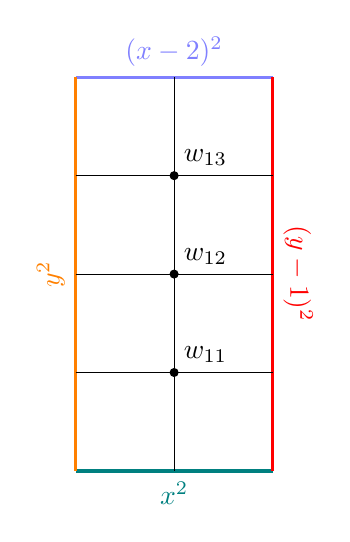
\begin{tikzpicture}[scale=2.5]
            \draw (0,0) rectangle (1,2);
            \draw[teal, very thick] (0,0) to node[below] {$x^2$} (1,0);
            \draw[blue!50, very thick] (0,2) to node[above] {$(x-2)^2$} (1,2);
            \draw[orange, very thick] (0,0) to node[left] {\rotatebox{90}{$y^2$}} (0,2);
            \draw[red, very thick] (1,0) to node[right] {\rotatebox{270}{$(y-1)^2$}} (1,2);
    
            \draw (0.5,0) -- (0.5,2);
    
            \draw (0, 0.5) -- (1, 0.5);
            \draw (0, 1.0) -- (1, 1.0);
            \draw (0, 1.5) -- (1, 1.5);
    
            \filldraw (0.5,0.5) circle (0.02) node[above right] {$w_{11}$};
            \filldraw (0.5,1.0) circle (0.02) node[above right] {$w_{12}$};
            \filldraw (0.5,1.5) circle (0.02) node[above right] {$w_{13}$};
        \end{tikzpicture}
    \end{minipage}
    \begin{minipage}{0.7\textwidth}
        \[
            2\left( \lambda + 1 \right) w_{ij} - w_{i-1 \, j} - w_{i+1 \, j} - \lambda \left( w_{i \, j-1} + w_{i \, j+1} \right) = -h^2 f(x_i, y_j)
        \]

        onde $\lambda = (k/h)^2$, nesse caso $h = k$, então $\lambda = 1$
    
        $i = 1$ e $j = 1$:
        \[
            4 w_{11} - \textcolor{orange}{w_{01}} - \textcolor{red}{w_{21}} - \textcolor{teal}{w_{10}} - w_{12} = -h^2 f(x_1, y_1)
        \]
    
        $i = 1$ e $j = 2$:
        \[
            4 w_{12} - \textcolor{orange}{w_{02}} - \textcolor{red}{w_{22}} - w_{11} - w_{13} = -h^2 f(x_1, y_2)
        \]
    
        $i = 1$ e $j = 3$:
        \[
            4 w_{13} - \textcolor{orange}{w_{03}} - \textcolor{red}{w_{23}} - w_{12} - \textcolor{blue!50}{w_{14}} = -h^2 f(x_1, y_3)
        \]
    \end{minipage}

    \medskip

    substituindo os valores ja conhecidos pelas condições de fronteira, temos o sistema
    \[
        \left\{ 
            \begin{array}{rlrlrl}
                4w_{11} &- &w_{12}  & &        &= -0.25 \\
                -w_{11} &+ &4w_{12} &- &w_{13} &= 0\\
                        &- &w_{12}  &+&4w_{13} &= 3.75
            \end{array}
        \right.
    \]

    com solução
    \[
        (w_{11}, w_{12}, w_{13}) = (0, 0.25, 1)
    \]
    e nesses pontos a solução real é
    \[
        (u(x_1, y_1), u(x_1, y_2), u(x_1, y_3)) = (0, 0.25, 1)
    \]
    

    \item Utilize o algoritmo 12.1 para determinar uma solução aproximada da equação diferencial parcial elíptica
    \[
        \dfrac{\partial^2 u}{\partial x^2} + \dfrac{\partial^2 u}{\partial y^2} = 0 \quad (x,y) \in [1,2] \times [0,1]
    \]
    com as condições
    \[
        \left\{  
            \begin{array}{ll}
                u(x,0) = 2 \ln x & x \in [1,2]\\  
                u(x,1) = \ln (x^2 + 1) & x \in [1,2]\\
                u(1,y) = \ln (y^2 + 1) & y \in [0,1]\\
                u(2,y) = \ln (y^2 + 4) & y \in [0,1]\\
            \end{array}
        \right.
    \]
    Use $h = k = \frac{1}{3}$ e compare os resultados com a solução real $u(x,y) = \ln (x^2 + y^2)$

    \begin{minipage}{0.35\columnwidth}
        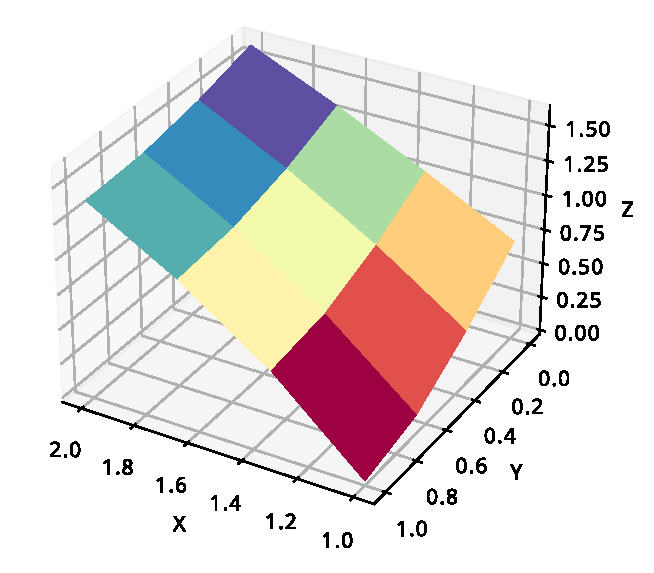
\includegraphics[width=\columnwidth]{../edp/12.1_2.pdf}
    \end{minipage}
    \begin{minipage}{0.6\columnwidth}
        \begin{align*}
            U_{\text{apr}} &= 
            \begin{bmatrix}
                0.693147 & 1.021651 & 1.329135 & 1.609437\\
                0.367724 & 0.798500 & 1.169820 & 1.491654\\
                0.105360 & 0.634804 & 1.059992 & 1.413693\\
                0.000000 & 0.575364 & 1.021651 & 1.386294\\
            \end{bmatrix}\\
            U_{\text{real}} &=
            \begin{bmatrix}
                0.693147 & 1.021651 & 1.329135 & 1.609437\\
                0.367724 & 0.798507 & 1.170071 & 1.491654\\
                0.105360 & 0.635988 & 1.060871 & 1.413693\\
                0.000000 & 0.575364 & 1.021651 & 1.386294\\
            \end{bmatrix}\\
            \text{erro} &= 
            \begin{bmatrix}
                0.000000 & 0.000000 & 0.000000 & 0.000000 \\
                0.000000 & 0.000007 & 0.000250 & 0.000000 \\
                0.000000 & 0.001184 & 0.000879 & 0.000000 \\
                0.000000 & 0.000000 & 0.000000 & 0.000000 \\
            \end{bmatrix}
        \end{align*}
    \end{minipage}

    \item Obtenha aproximações para as soluções das operações diferenciais parciais elípticas seguintes
    \begin{enumerate}[leftmargin=*, label=\alph*.]
        \item ~
        \[
        \dfrac{\partial^2 u}{\partial x^2} + \dfrac{\partial^2 u}{\partial y^2} = 0 \quad (x,y) \in [0,1] \times [0,1]
        \]
        com as condições
        \[
            \left\{  
                \begin{array}{ll}
                    u(x,0) = 0 & x \in [0,1]\\  
                    u(x,2) = x & x \in [0,1]\\
                    u(0,y) = 0 & y \in [0,1]\\
                    u(1,y) = y & y \in [0,1]\\
                \end{array}
            \right.
        \]
        Use $h = k = 0.2$ e compare os resultados com a solução real $u(x,y) = xy$
        
        \begin{minipage}{0.35\columnwidth}
            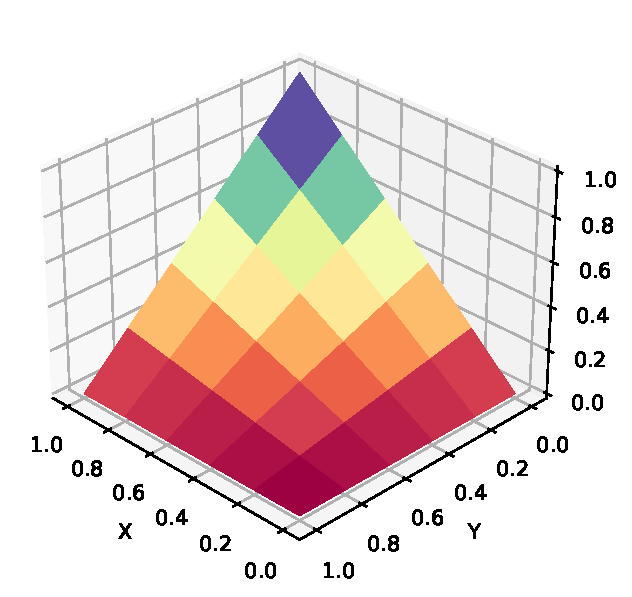
\includegraphics[width=\columnwidth]{../edp/12.1_3a.pdf}
        \end{minipage}
        \begin{minipage}{0.6\columnwidth}
            \begin{align*}
                U_{\text{apr}} &= 
                \begin{bmatrix}
                    0.00 & 0.20 & 0.40 & 0.60 & 0.80 & 1.00\\ 
                    0.00 & 0.16 & 0.32 & 0.48 & 0.64 & 0.80 \\ 
                    0.00 & 0.12 & 0.24 & 0.36 & 0.48 & 0.60 \\ 
                    0.00 & 0.08 & 0.16 & 0.24 & 0.32 & 0.40 \\ 
                    0.00 & 0.04 & 0.08 & 0.12 & 0.16 & 0.20 \\ 
                    0.00 & 0.00 & 0.00 & 0.00 & 0.00 & 0.00 \\ 
                \end{bmatrix}\\
                U_{\text{real}} &=
                \begin{bmatrix}
                    0.00 & 0.20 & 0.40 & 0.60 & 0.80 & 1.00\\ 
                    0.00 & 0.16 & 0.32 & 0.48 & 0.64 & 0.80 \\ 
                    0.00 & 0.12 & 0.24 & 0.36 & 0.48 & 0.60 \\ 
                    0.00 & 0.08 & 0.16 & 0.24 & 0.32 & 0.40 \\ 
                    0.00 & 0.04 & 0.08 & 0.12 & 0.16 & 0.20 \\ 
                    0.00 & 0.00 & 0.00 & 0.00 & 0.00 & 0.00 \\
                \end{bmatrix}\\
                \text{erro} &= 
                \begin{bmatrix}
                    0.00 & 0.00 & 0.00 & 0.00 & 0.00 & 0.00 \\
                    0.00 & 0.00 & 0.00 & 0.00 & 0.00 & 0.00 \\
                    0.00 & 0.00 & 0.00 & 0.00 & 0.00 & 0.00 \\
                    0.00 & 0.00 & 0.00 & 0.00 & 0.00 & 0.00 \\
                    0.00 & 0.00 & 0.00 & 0.00 & 0.00 & 0.00 \\
                    0.00 & 0.00 & 0.00 & 0.00 & 0.00 & 0.00 \\
                \end{bmatrix}
            \end{align*}
        \end{minipage}

        \item ~
        \[
        \dfrac{\partial^2 u}{\partial x^2} + \dfrac{\partial^2 u}{\partial y^2} = -\cos (x+y) - \cos (x-y) \quad (x,y) \in [0,\pi] \times [0,\tfrac{\pi}{2}]
        \]
        com as condições
        \[
            \left\{  
                \begin{array}{ll}
                    u(x,0) = \cos x & x \in [0,\pi]\\  
                    u(x,\frac{\pi}{2}) = 0 & x \in [0,\pi]\\
                    u(0,y) = \cos y & y \in [0,\frac{\pi}{2}]\\
                    u(\pi,y) = -\cos y & y \in [0,\frac{\pi}{2}]\\
                \end{array}
            \right.
        \]
        Use $h = \frac{\pi}{5}$, $k = \frac{\pi}{10}$ e compare os resultados com a solução real $u(x,y) = xy$
        
        \begin{minipage}{0.35\columnwidth}
            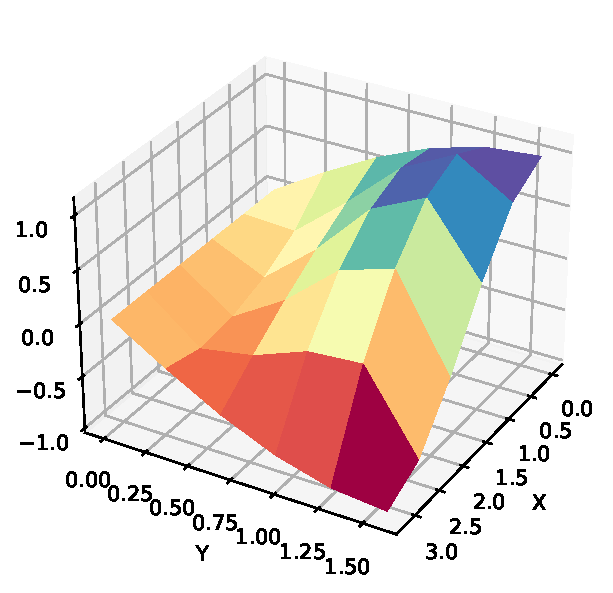
\includegraphics[width=\columnwidth]{../edp/12.1_3b.pdf}
        \end{minipage}
        \begin{minipage}{0.6\columnwidth}
            \begin{align*}
                U_{\text{apr}} &= 
                {\small
                \begin{bmatrix}
                    0.000 &  0.000 &  0.000 &  0.000 &  0.000 &  0.000\\
                    0.309 & -0.026 & -0.229 & -0.349 & -0.391 & -0.309\\
                    0.587 &  0.393 &  0.189 & -0.040 & -0.301 & -0.587\\
                    0.809 &  0.855 &  0.709 &  0.389 & -0.107 & -0.809\\
                    0.951 &  1.113 &  0.951 &  0.547 & -0.067 & -0.951\\
                    1.000 &  0.809 &  0.309 & -0.309 & -0.809 & -1.000\\     
                \end{bmatrix}}\\
                U_{\text{real}} &=
                {\small
                \begin{bmatrix}
                    0.000 & 0.000 & 0.000 & 0.000 & 0.000 & 0.000 \\
                    0.309 & 0.250 & 0.095 &-0.095 &-0.250 &-0.309 \\
                    0.587 & 0.475 & 0.181 &-0.181 &-0.475 &-0.587 \\
                    0.809 & 0.654 & 0.250 &-0.250 &-0.654 &-0.809 \\
                    0.951 & 0.769 & 0.293 &-0.293 &-0.769 &-0.951 \\
                    1.000 & 0.809 & 0.309 &-0.309 &-0.809 &-1.000 \\
                \end{bmatrix}}\\
                \text{erro} &= 
                \begin{bmatrix}
                    0.000 & 0.000 & 0.000 & 0.000 & 0.000 & 0.000 \\
                    0.000 & 0.276 & 0.324 & 0.254 & 0.141 & 0.000 \\
                    0.000 & 0.081 & 0.007 & 0.140 & 0.174 & 0.000 \\
                    0.000 & 0.201 & 0.459 & 0.639 & 0.547 & 0.000 \\
                    0.000 & 0.343 & 0.657 & 0.841 & 0.701 & 0.000 \\
                    0.000 & 0.000 & 0.000 & 0.000 & 0.000 & 0.000 \\
                \end{bmatrix}
            \end{align*}
        \end{minipage}
    \end{enumerate}
\end{enumerate}

\section{Equações parabólicas}
\begin{enumerate}[leftmargin=*]
    \item Determine uma aproximação para a solução da equação diferencial seguinte utilizando o método das diferenças regressivas
    \[
        \dfrac{\partial u}{\partial t} - \dfrac{\partial^2 u}{\partial y^2} = 0 \quad 0 < x < 2, \, 0 < t
        \]
        com as condições
        \[
            \left\{  
                \begin{array}{ll}
                    u(x,0) = \sin \frac{\pi}{2} x & x \in [0,2]\\  
                    u(0,t) = 0 & 0 < t\\
                    u(2,t) = 0 & 0 < t\\
                \end{array}
            \right.
        \]
        Use $m = 4$, $T = 0.1$ e $N = 2$ e compare seus resultados com a solução real $u(x,t) = \exp\left(-\frac{\pi^2}{4}t\right)\sin \frac{\pi}{2}x$
        
        \begin{minipage}{0.35\columnwidth}
            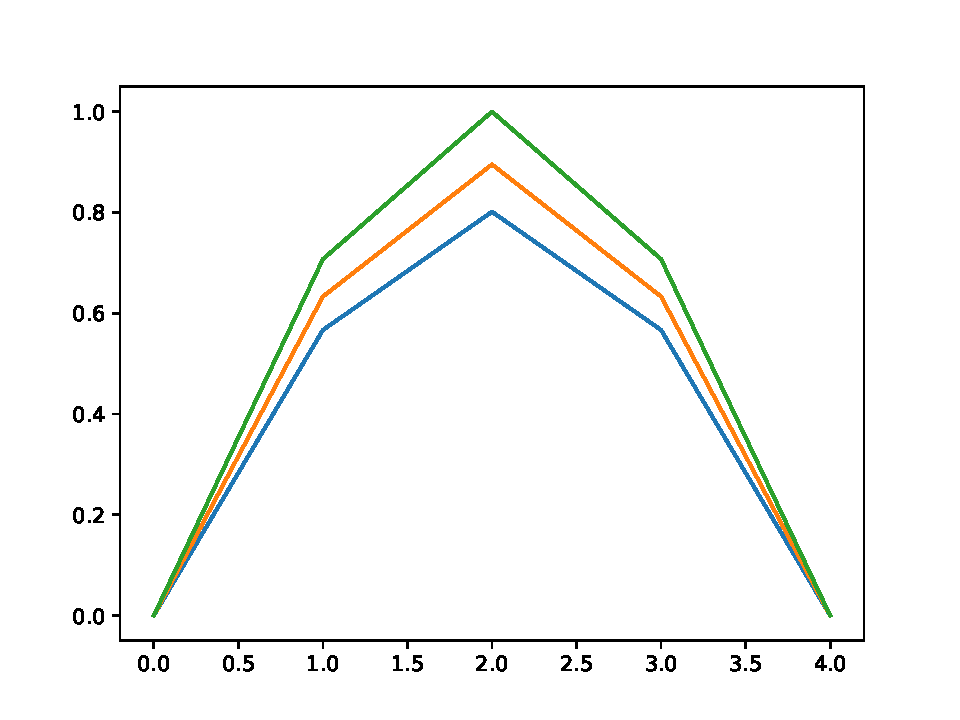
\includegraphics[width=\columnwidth]{../edp/12.2_1.pdf}
        \end{minipage}
        \begin{minipage}{0.6\columnwidth}
            \begin{align*}
                U_{\text{apr}} &= 
                \begin{bmatrix}
                    0.00000 & 0.56657 &  0.80126 &  0.56657 &  0.00000\\  
                    0.00000 & 0.63295 &  0.89513 &  0.63295 &  0.00000\\  
                    0.00000 & 0.70711 &  1.00000 &  0.70711 &  0.00000\\  
                \end{bmatrix}\\
                U_{\text{real}} &=
                \begin{bmatrix}
                    0.00000  & 0.55249 &  0.78134 &  0.55249 &  0.00000\\  
                    0.00000  & 0.62504 &  0.88394 &  0.62504 &  0.00000\\  
                    0.00000  & 0.70711 &  1.00000 &  0.70711 &  0.00000\\ 
                \end{bmatrix}\\
                \text{erro} &= 
                \begin{bmatrix}
                    0.00000 &  0.01408 &  0.01991 &  0.01408 &  0.00000\\  
                    0.00000 &  0.00791 &  0.01119 &  0.00791 &  0.00000\\  
                    0.00000 &  0.00000 &  0.00000 &  0.00000 &  0.00000\\ 
                \end{bmatrix}
            \end{align*}
        \end{minipage}
        \item Determine uma aproximação para a solução da equação diferencial seguinte utilizando o método das diferenças regressivas
        \[
        \dfrac{\partial u}{\partial t} - \frac{1}{16}\dfrac{\partial^2 u}{\partial y^2} = 0 \quad 0 < x < 1, \, 0 < t
        \]
        com as condições
        \[
            \left\{  
                \begin{array}{ll}
                    u(x,0) = 2\sin 2\pi x & x \in [0,1]\\  
                    u(0,t) = 0 & 0 < t\\
                    u(1,t) = 0 & 0 < t\\
                \end{array}
            \right.
        \]
        Use $m = 3$, $T = 0.1$ e $N = 2$ e compare seus resultados com a solução real $u(x,t) = 2e^{-\frac{\pi^2t}{4}}\sin 2 \pi x$
        
        \begin{minipage}{0.35\columnwidth}
            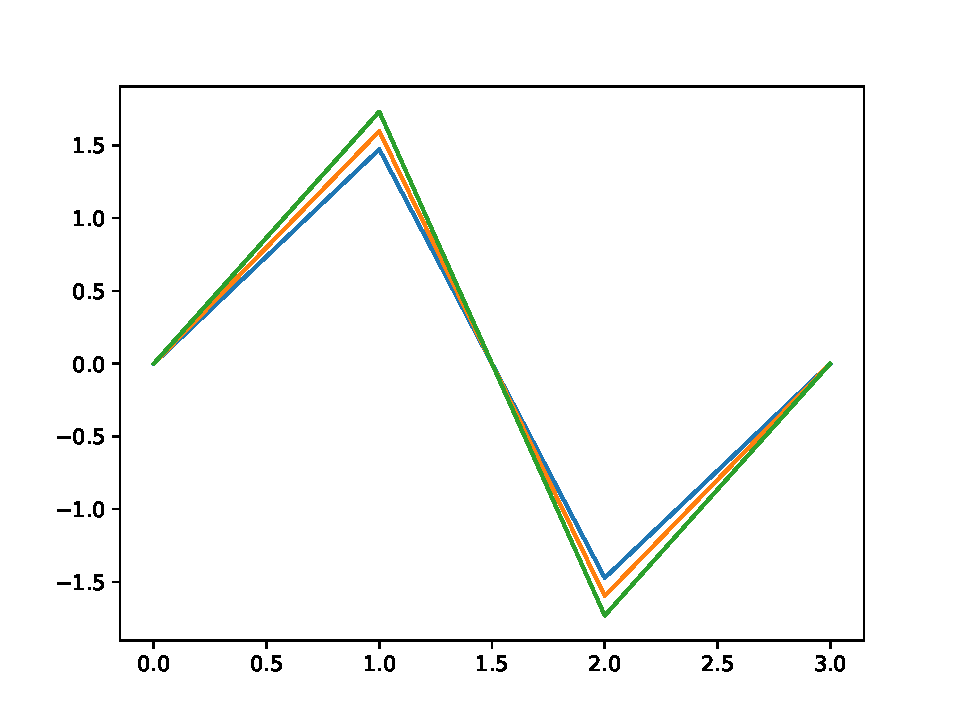
\includegraphics[width=\columnwidth]{../edp/12.2_2.pdf}
        \end{minipage}
        \begin{minipage}{0.6\columnwidth}
            \begin{align*}
                U_{\text{apr}} &= 
                \begin{bmatrix}
                    0.00000 & 1.47300 & -1.47300 &  0.00000\\  
                    0.00000 & 1.59728 & -1.59728 &  0.00000\\  
                    0.00000 & 1.73205 & -1.73205 &  0.00000\\
                \end{bmatrix}\\
                U_{\text{real}} &=
                \begin{bmatrix}
                    0.00000 &  1.35333 &  -1.35333  & 0.00000\\  
                    0.00000 &  1.53102 &  -1.53102  & 0.00000\\  
                    0.00000 &  1.73205 &  -1.73205  & 0.00000\\ 
                \end{bmatrix}\\
                \text{erro} &= 
                \begin{bmatrix}
                    0.00000 & 0.11967 &  0.11967 &  0.00000\\  
                    0.00000 & 0.06626 &  0.06626 &  0.00000\\  
                    0.00000 & 0.00000 &  0.00000 &  0.00000\\  
                \end{bmatrix}
            \end{align*}
        \end{minipage}
        \item[5.] Utilize o método das diferenças progressívas para obter uma aproximação para a solução das equação diferencial parcial seguinte
        \[
        \dfrac{\partial u}{\partial t} - \dfrac{\partial^2 u}{\partial y^2} = 0 \quad 0 < x < 2, \, 0 < t
        \]
        com as condições
        \[
            \left\{  
                \begin{array}{ll}
                    u(x,0) = \sin 2\pi x & x \in [0,2]\\  
                    u(0,t) = 0 & 0 < t\\
                    u(2,t) = 0 & 0 < t\\
                \end{array}
            \right.
        \]
        Use $h = 0.4$, $k = 0.1$ e compare seus resultados em $t = 0.5$ com a solução real $u(x,t) = e^{-4\pi^2t}\sin 2 \pi x$. A seguir, use $k = 0.05$ e compare suas respostas
        
        \begin{minipage}{0.35\columnwidth}
            \begin{center}
                com $k = 0.1$
            \end{center}
            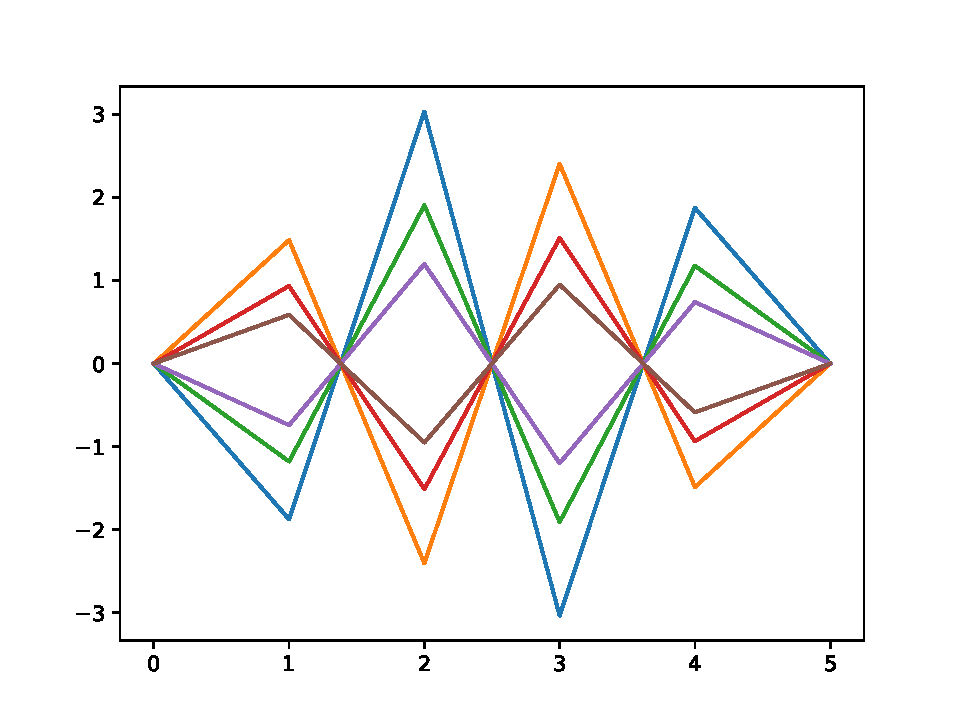
\includegraphics[width=\columnwidth]{../edp/12.2_5a1.pdf}
        \end{minipage}
        \begin{minipage}{0.6\columnwidth}
            \begin{align*}
                U_{\text{apr}} &= 
                {\small
                \begin{bmatrix}
                    0.00000 & -1.87612 &   3.03563 &  -3.03563 &  1.87612  & 0.00000\\  
                    0.00000 &  1.48749 &  -2.40680 &   2.40680 & -1.48749  & 0.00000\\  
                    0.00000 & -1.17935 &   1.90823 &  -1.90823 &  1.17935  & 0.00000\\  
                    0.00000 &  0.93505 &  -1.51295 &   1.51295 & -0.93505  & 0.00000\\  
                    0.00000 & -0.74136 &   1.19954 &  -1.19954 &  0.74136  & 0.00000\\  
                    0.00000 &  0.58779 &  -0.95106 &   0.95106 & -0.58779  & 0.00000\\ 
                \end{bmatrix}}\\
                U_{\text{real}} &=
                {\small
                \begin{bmatrix}
                    0.00000 &  0.00000 & -0.00000 &  0.00000 & -0.00000 & 0.00000\\  
                    0.00000 &  0.00000 & -0.00000 &  0.00000 & -0.00000 & 0.00000\\  
                    0.00000 &  0.00000 & -0.00001 &  0.00001 & -0.00000 & 0.00000\\  
                    0.00000 &  0.00022 & -0.00035 &  0.00035 & -0.00022 & 0.00000\\  
                    0.00000 &  0.01134 & -0.01835 &  0.01835 & -0.01134 & 0.00000\\  
                    0.00000 &  0.58779 & -0.95106 &  0.95106 & -0.58779 & 0.00000\\ 
                \end{bmatrix}}\\
                \text{erro} &= 
                {\small
                \begin{bmatrix}
                    0.00000 &  1.87612  & 3.03563 &  3.03563  & 1.87612  & 0.00000 \\ 
                    0.00000 &  1.48749  & 2.40680 &  2.40680  & 1.48749  & 0.00000 \\ 
                    0.00000 &  1.17936  & 1.90824 &  1.90824  & 1.17936  & 0.00000 \\ 
                    0.00000 &  0.93483  & 1.51259 &  1.51259  & 0.93483  & 0.00000 \\ 
                    0.00000 &  0.75270  & 1.21789 &  1.21789  & 0.75270  & 0.00000 \\ 
                    0.00000 &  0.00000  & 0.00000 &  0.00000  & 0.00000  & 0.00000 \\
                \end{bmatrix}}
            \end{align*}
        \end{minipage}

        \begin{minipage}{0.35\columnwidth}
            \begin{center}
                com $k = 0.05$
            \end{center}
            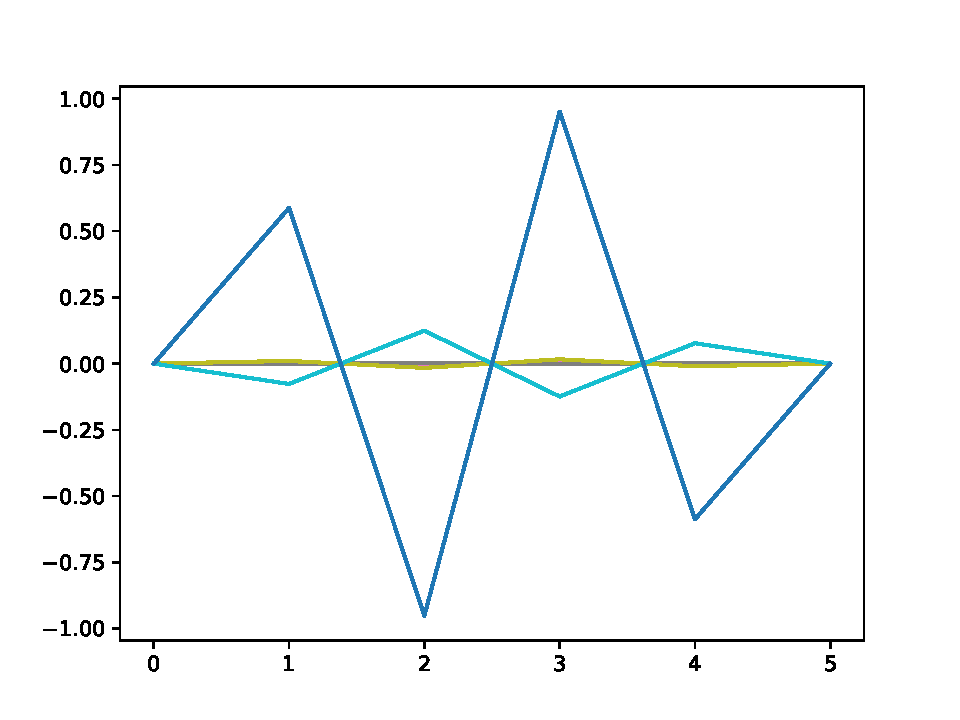
\includegraphics[width=\columnwidth]{../edp/12.2_5a2.pdf}
        \end{minipage}
        \begin{minipage}{0.6\columnwidth}
            \begin{align*}
                U_{\text{apr}} &= 
                {\small
                \begin{bmatrix}
                    0.00000 &   0.00000 &  -0.00000 &   0.00000 &  -0.00000 &   0.00000\\  
                    0.00000 &  -0.00000 &   0.00000 &  -0.00000 &   0.00000 &   0.00000\\  
                    0.00000 &   0.00000 &  -0.00000 &   0.00000 &  -0.00000 &   0.00000\\  
                    0.00000 &  -0.00000 &   0.00000 &  -0.00000 &   0.00000 &   0.00000\\  
                    0.00000 &   0.00000 &  -0.00000 &   0.00000 &  -0.00000 &   0.00000\\  
                    0.00000 &  -0.00002 &   0.00004 &  -0.00004 &   0.00002 &   0.00000\\  
                    0.00000 &   0.00017 &  -0.00028 &   0.00028 &  -0.00017 &   0.00000\\  
                    0.00000 &  -0.00131 &   0.00212 &  -0.00212 &   0.00131 &   0.00000\\  
                    0.00000 &   0.01003 &  -0.01623 &   0.01623 &  -0.01003 &   0.00000\\  
                    0.00000 &  -0.07679 &   0.12424 &  -0.12424 &   0.07679 &   0.00000\\  
                    0.00000 &   0.58779 &  -0.95106 &   0.95106 &  -0.58779 &   0.00000\\  
                \end{bmatrix}}\\
                U_{\text{real}} &=
                {\small
                \begin{bmatrix}
                    0.00000 &  0.00000 & -0.00000 &  0.00000 &  -0.00000  & 0.00000 \\  
                    0.00000 &  0.00000 & -0.00000 &  0.00000 &  -0.00000  & 0.00000 \\  
                    0.00000 &  0.00000 & -0.00000 &  0.00000 &  -0.00000  & 0.00000 \\  
                    0.00000 &  0.00000 & -0.00000 &  0.00000 &  -0.00000  & 0.00000 \\  
                    0.00000 &  0.00000 & -0.00001 &  0.00001 &  -0.00000  & 0.00000 \\  
                    0.00000 &  0.00003 & -0.00005 &  0.00005 &  -0.00003  & 0.00000 \\  
                    0.00000 &  0.00022 & -0.00035 &  0.00035 &  -0.00022  & 0.00000 \\  
                    0.00000 &  0.00158 & -0.00255 &  0.00255 &  -0.00158  & 0.00000 \\  
                    0.00000 &  0.01134 & -0.01835 &  0.01835 &  -0.01134  & 0.00000 \\  
                    0.00000 &  0.08165 & -0.13211 &  0.13211 &  -0.08165  & 0.00000 \\  
                    0.00000 &  0.58779 & -0.95106 &  0.95106 &  -0.58779  & 0.00000 \\ 
                \end{bmatrix}}\\
                \text{erro} &= 
                {\small
                \begin{bmatrix}
                    0.00000  & 0.00000  & 0.00000 &  0.00000  & 0.00000  & 0.00000  \\
                    0.00000  & 0.00000  & 0.00000 &  0.00000  & 0.00000  & 0.00000  \\
                    0.00000  & 0.00000  & 0.00000 &  0.00000  & 0.00000  & 0.00000  \\
                    0.00000  & 0.00000  & 0.00000 &  0.00000  & 0.00000  & 0.00000  \\
                    0.00000  & 0.00000  & 0.00000 &  0.00000  & 0.00000  & 0.00000  \\
                    0.00000  & 0.00005  & 0.00009 &  0.00009  & 0.00005  & 0.00000  \\
                    0.00000  & 0.00005  & 0.00008 &  0.00008  & 0.00005  & 0.00000  \\
                    0.00000  & 0.00289  & 0.00467 &  0.00467  & 0.00289  & 0.00000  \\
                    0.00000  & 0.00131  & 0.00212 &  0.00212  & 0.00131  & 0.00000  \\
                    0.00000  & 0.15844  & 0.25635 &  0.25635  & 0.15844  & 0.00000  \\
                    0.00000  & 0.00000  & 0.00000 &  0.00000  & 0.00000  & 0.00000  \\
                \end{bmatrix}}
            \end{align*}
        \end{minipage}
        
\end{enumerate}
\section{Equações hiperbólicas}
\begin{enumerate}[leftmargin=*]
    \item Determine uma aproximação para a solução da equação diferencial seguinte utilizando o método das diferenças regressivas
    \[
    \dfrac{\partial u}{\partial t} - \dfrac{\partial^2 u}{\partial y^2} = 0 \quad 0 < x < 2, \, 0 < t
    \]
    com as condições
    \[
        \left\{  
            \begin{array}{ll}
                u(x,0) = \sin \pi x & x \in [0,1]\\  
                u(0,t) = 0 & 0 < t\\
                u(1,t) = 0 & 0 < t\\
                u_t(x,0) = 0 & x \in [0,1]
            \end{array}
        \right.
    \]
    Use $m = 4$, $T = 1$ e $N = 4$ e compare seus resultados com a solução real $u(x,t) = cos \pi t \, \sin \pi x$
    
    \begin{minipage}{0.35\columnwidth}
        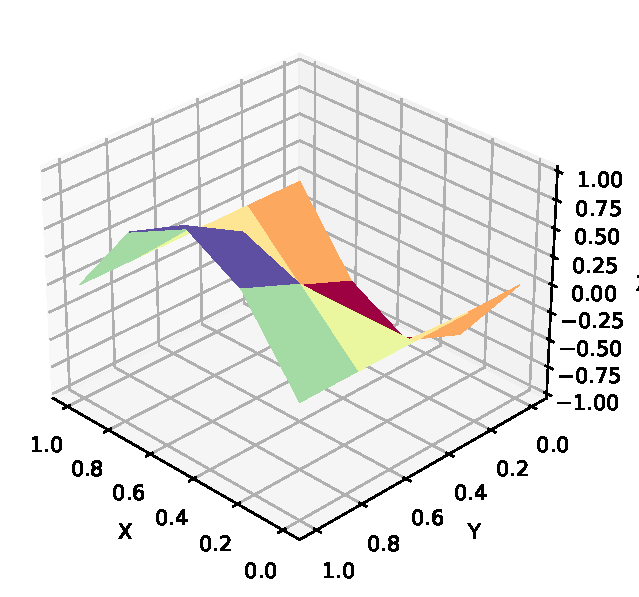
\includegraphics[width=\columnwidth]{../edp/12.3_1.pdf}
    \end{minipage}
    \begin{minipage}{0.6\columnwidth}
        \begin{align*}
            U_{\text{apr}} &= 
            \begin{bmatrix}
                0.00000 & -0.70711 &  -1.00000 &  -0.70711 &  0.00000\\  
                0.00000 & -0.50000 &  -0.70711 &  -0.50000 &  0.00000\\  
                0.00000 &  0.00000 &   0.00000 &   0.00000 &  0.00000\\  
                0.00000 &  0.50000 &   0.70711 &   0.50000 &  0.00000\\  
                0.00000 &  0.70711 &   1.00000 &   0.70711 &  0.00000\\    
            \end{bmatrix}\\
            U_{\text{real}} &=
            \begin{bmatrix}
                0.00000 & -0.70711 & -1.00000 &  -0.70711 &  0.00000\\  
                0.00000 & -0.50000 & -0.70711 &  -0.50000 &  0.00000\\  
                0.00000 &  0.00000 &  0.00000 &   0.00000 &  0.00000\\  
                0.00000 &  0.50000 &  0.70711 &   0.50000 &  0.00000\\  
                0.00000 &  0.70711 &  1.00000 &   0.70711 &  0.00000\\
            \end{bmatrix}\\
            \text{erro} &= 
            \begin{bmatrix}
                0.00000 & 0.00000 &  0.00000 &  0.00000 &  0.00000\\  
                0.00000 & 0.00000 &  0.00000 &  0.00000 &  0.00000\\  
                0.00000 & 0.00000 &  0.00000 &  0.00000 &  0.00000\\  
                0.00000 & 0.00000 &  0.00000 &  0.00000 &  0.00000\\  
                0.00000 & 0.00000 &  0.00000 &  0.00000 &  0.00000\\  
            \end{bmatrix}
        \end{align*}
    \end{minipage}
    \item Determine uma aproximação para a solução da equação diferencial seguinte utilizando o método das diferenças regressivas
    \[
    \dfrac{\partial u}{\partial t} - \frac{1}{16\pi^2}\dfrac{\partial^2 u}{\partial y^2} = 0 \quad 0 < x < 0.5, \, 0 < t
    \]
    com as condições
    \[
        \left\{  
            \begin{array}{ll}
                u(x,0) = \sin \frac{\pi}{2} x & x \in [0,0.5]\\  
                u(0,t) = 0 & 0 < t\\
                u(0.5,t) = 0 & 0 < t\\
                u_t(x,0) = \sin 4 \pi x & x \in [0,0.5]
            \end{array}
        \right.
    \]
    Use $m = 4$, $T = 0.5$ e $N = 4$ e compare seus resultados com a solução real $u(x,t) = \sin t \, \sin 4\pi x$
    
    \begin{minipage}{0.35\columnwidth}
        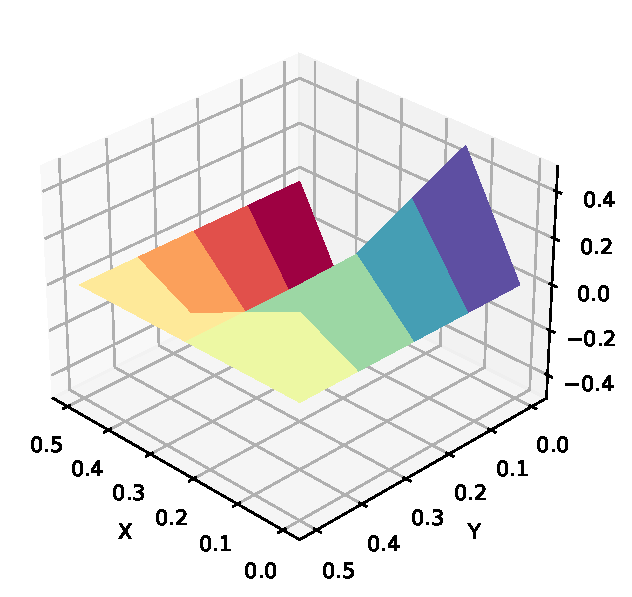
\includegraphics[width=\columnwidth]{../edp/12.3_2.pdf}
    \end{minipage}
    \begin{minipage}{0.6\columnwidth}
        \begin{align*}
            U_{\text{apr}} &= 
            \begin{bmatrix}
                0.00000 &   0.48429  & 0.00000  & -0.48429  & 0.00000\\ 
                0.00000 &   0.36869  & 0.00000  & -0.36869  & 0.00000\\ 
                0.00000 &   0.24842  & 0.00000  & -0.24842  & 0.00000\\ 
                0.00000 &   0.12500  & 0.00000  & -0.12500  & 0.00000\\ 
                0.00000 &   0.00000  & 0.00000  &  0.00000  & 0.00000\\
            \end{bmatrix}\\
            U_{\text{real}} &=
            \begin{bmatrix}
                0.00000 &  0.47943 &  0.00000 &  -0.47943  & -0.00000  \\
                0.00000 &  0.36627 &  0.00000 &  -0.36627  & -0.00000  \\
                0.00000 &  0.24740 &  0.00000 &  -0.24740  & -0.00000  \\
                0.00000 &  0.12467 &  0.00000 &  -0.12467  & -0.00000  \\
                0.00000 &  0.00000 &  0.00000 &  -0.00000  & -0.00000  \\
            \end{bmatrix}\\
            \text{erro} &= 
            \begin{bmatrix}
                0.00000  & 0.00486  & 0.00000  & 0.00486 &  0.00000\\  
                0.00000  & 0.00241  & 0.00000  & 0.00241 &  0.00000\\  
                0.00000  & 0.00101  & 0.00000  & 0.00101 &  0.00000\\  
                0.00000  & 0.00033  & 0.00000  & 0.00033 &  0.00000\\  
                0.00000  & 0.00000  & 0.00000  & 0.00000 &  0.00000\\  
            \end{bmatrix}
        \end{align*}
    \end{minipage}
\end{enumerate}
\end{document}